\documentclass[11pt]{article}
% Proc. R. Soc. B research article, anonymised for double-anonymous review (author details in title_page.tex)
\usepackage[a4paper,margin=2.5cm]{geometry}
\usepackage[utf8]{inputenc}
\usepackage[T1]{fontenc}
\usepackage{lmodern}
\usepackage{amsmath}
\usepackage{graphicx}
\usepackage{setspace}
\usepackage[numbers,sort&compress,square]{natbib}
\usepackage[hidelinks]{hyperref}
\usepackage{lineno}
\usepackage{caption}
\captionsetup{font=small,labelfont=bf,labelsep=period}
\onehalfspacing
\linenumbers

\title{What comes first, connectivity or homophily? From chimpanzees to prehistoric villages}
\author{}
\date{}

\begin{document}
\maketitle

\begin{abstract}
\noindent
Communities in human and animal societies are usually attributed to homophily, the tendency of similar
individuals to bond. Local network growth offers an alternative: when ties form through friends of
friends, connectivity alone partitions a population, and shared traits can follow. The two mechanisms
leave similar traces in a snapshot. Using 15,260 synthetic societies, we show that snapshot statistics
cannot separate them at the sizes of ancestral groups, and reverse when traits spread along ties,
whereas temporal order can. We then examine four records. Sex and age predict neither the fission of the
Ngogo chimpanzee community nor support ties in two small-scale human societies; the fission follows
ranging areas, and Mayangna support follows the genealogical network beyond pairwise relatedness. In
prehistoric Central Europe, shared archaeological culture and genetic kinship are coupled beyond
geography. In three centuries of Chaco ceramic exchange, settlements in the same community became more
similar over the following 50--100 years, whereas the time-reversed effect is absent ($P<0.002$ against
a stationary null). Network structure often precedes similarity, and the two act together in shaping
communities.
\end{abstract}

\noindent\textbf{Keywords:} homophily, social networks, community structure, cultural evolution,
archaeological networks

%======================================================================
\section{Introduction}

Why do societies split into groups? The dominant answer in the social sciences is homophily: like
attracts like, and communities are the visible trace of shared kinship, language, ethnicity, status or
belief~\cite{McPherson2001}. The answer has been projected into deep time. Models of cultural evolution
propose that marking group identity with arbitrary symbols became adaptive because it let individuals
find partners with compatible norms~\cite{McElreath2003}, implying that homophily was a founding force of
early human social structure.

Network science points to a different mechanism. Social ties are rarely formed at random: people meet
the friends of their friends, the kin of their kin, the neighbours of their neighbours. When networks
grow by such local rules, through triadic closure, local search or duplication of an existing node's
ties, the growth process itself produces tightly knit groups loosely connected to each
other~\cite{Jin2001,Vazquez2003,Toivonen2006}. No node needs to differ from any other. Communities then
encode the history of the network rather than the traits of its members. For the simplest local rules,
these communities become statistically detectable only above a characteristic size $r_\kappa$ of about
80 to 100 nodes~\cite{VazquezBook}, close to the size of many forager bands and early villages.

The two mechanisms are hard to tell apart. In a single snapshot, homophily (similar individuals bond)
and social contagion (bonded individuals become similar) produce the same correlation between ties and
traits~\cite{Shalizi2011}. Spatial proximity mimics both. And kinship, the most important trait in
small-scale societies, is itself a network, a genealogy grown by local rules. Testing the origin of
communities in early societies therefore requires two things: knowing which statistics discriminate
between the mechanisms at realistic group sizes, and data that offer either a natural experiment or a
time series.

We address both. We first grow 15,260 synthetic societies in which a tunable share of ties is placed by
homophily and the rest by local network growth, and determine which signatures recover that share at
sizes from 20 to 500 individuals. We then apply the informative signatures to four bodies of evidence
spanning primate, ethnographic and archaeological time scales: the fission of a chimpanzee community,
support networks in two small-scale human societies, kinship networks from ancient genomes, and a
three-century time series of ceramic exchange.

%======================================================================
\section{Material and methods}

All analyses use previously published, public data, cited below. Code and derived results for every
analysis are provided as electronic supplementary material.

\subsection{Synthetic societies}
Networks grow by adding one node with two links per step. In the local-search model LS$(n,1)$ the first
link goes to a uniformly chosen anchor and the second to a random neighbour of the anchor (triadic
closure); in the duplication--split model DS$(n,0.5)$ a newcomer copies and splits the links of an
existing node~\cite{VazquezBook}. A mixing share $\lambda$ of links (LS) or newcomers (DS) is instead
placed by homophily: with probability $h=0.8$ the target is restricted to the newcomer's type ($K=2$
balanced types) and chosen in proportion to degree plus one, giving 90\% within-type ties and comparable
degree distributions~\cite{Karimi2018}. Thus $\lambda=0$ is pure connectivity and $\lambda=1$ pure
homophily. Controls are a static attribute block model, a spatial model (positions in the unit square,
links $\propto e^{-d/0.1}$, attribute given by side), and preferential attachment without types. In the
contagion scenario two nodes per step copy a neighbour's type (probability $1-\lambda$) or redraw it
(probability $\lambda$). Dense similarity-type networks keep the 90\% of pairs closest in graph distance.
Sizes were $n=20$--500 with 60 replicates per condition (15,260 networks), with sensitivity runs at
$h=0.5$ and 0.95, $K=4$, and eight latent types of which two classes are observed.

The statistics were: alignment (normalised mutual information, NMI, and adjusted Rand index, ARI)
between the degree-corrected stochastic block model (DC-SBM) partition~\cite{Peixoto2014} and the type;
the description-length gain of the type partition; a dyadic logit of ties on same type, common
neighbours, log degrees and distance; partition agreement across replicate histories; agreement of a
simulated fission cut with the type; and, as temporal statistics, convergence of traits after a tie forms
and type selection at tie formation. Power is the area under the receiver operating characteristic curve
(AUC) for separating $\lambda=0$ from $\lambda=1$ societies. With $K$ balanced types, within-type edge
fraction $p$ and mean degree $\langle k\rangle$, homophily blocks are detectable only if
\begin{equation}
\frac{\langle k\rangle}{2}\left[p\ln(pK)+(1-p)\ln\frac{(1-p)K}{K-1}\right]>\ln K ,
\label{eq:detect}
\end{equation}
independently of $n$, which accounts for the weak power of community-alignment tests in sparse networks.
Closure beyond observed types also arises from homophily on unobserved types, which we treat as a
limitation of all snapshot tests.

\subsection{Ngogo chimpanzees}
We used the published learned weighted networks (grooming, proximity and party association; monthly,
1998--2022), post-fission group labels and the GPS subsample with sex and birth year~\cite{Sandel2026,NgogoData}.
Edges were $\log(1+w)$ summed over the window; analyses used the giant component (126 individuals in
2011--2014, 90 with a post-fission label). Unsupervised cuts were the Fiedler vector of the normalised
Laplacian and the leading modularity eigenvector, compared with 1,000 label permutations. Supervised
predictions used leave-one-out logistic regression on network features (Fiedler coordinate; weighted
neighbour vote with the focal label hidden), sex and age (with age squared and interaction), and median
GPS position, with permutation nulls. Within-sex cuts used sex-specific subgraphs. The post-fission
labels are themselves derived from the post-split network, and individuals who died before 2018 are
unlabelled.

For the matched-space test we used individuals with at least 30 GPS fixes in 2011--2014 (83 in the
grooming layer, 67 labelled). Home-range overlap is the Bhattacharyya affinity of Gaussian kernel
density estimates (bandwidth 300 m, 100-m grid). Pairs of labelled individuals were stratified by
overlap decile, decile of distance between median locations, and sex combination; within each stratum we
took the difference in mean $\log(1+w)$ between future groupmates and cross-line pairs, and averaged
across strata weighted by the smaller group. Intervals come from 500 node-bootstrap resamples.

\subsection{Human support networks}
Arang Dak: undirected ties are any report of monthly tangible support between adults of different
households (5,594 dyads); attributes are sex, age, wealth, consanguineal and affinal relatedness,
godparenthood and inter-household distance~\cite{Koster2018,KosterData}. Agta: directed gifts in a sharing game,
with sex, age, kin category, household proximity and need; the game's cooperation score is endogenous
and was excluded~\cite{Smith2018Agta,AgtaData}. Hadza: friendship nominations and GPS proximity in camps of 33 and
38~\cite{Fedurek2024,HadzaData}. Ties were predicted with L2-regularised logistic regression under repeated
five-fold cross-validation over dyads; network features (degree with the dyad's own tie removed, common
neighbours, Adamic--Adar, Jaccard, reciprocity, SBM block scores) were recomputed from training ties
only. DC-SBM partitions were compared with households, sex, age, spatial clusters and blocks of the
kinship graph by NMI against 1,000 permutations.

Kinship as a network (Arang Dak) entered as the number of common kin ($r\ge0.125$), the kin-weighted
two-path sums $\sum_k r_{ik}r_{kj}$ for consanguineal and affinal relatedness, and the path length in
the kin graph with co-residents linked (capped at 5). Common support partners were split by whether the
intermediary is related ($r\ge0.0625$ or affinal $r\ge0.0625$) to, or co-resident with, either member of
the pair. Increments were evaluated on identical folds (five folds, five repetitions).

\subsection{Ancient genomes}
IBD segments were taken from the ancIBD release for 4,248 ancient Eurasians~\cite{Ringbauer2024,ancIBDData}, with
metadata from the Allen Ancient DNA Resource~\cite{Mallick2024,AADRData}. We kept individuals older than 2000 BP
in 45--55$^\circ$N, 8--24$^\circ$E (705 individuals, 203 localities) and defined a tie as at least one
segment $\ge12$ cM. Culture was assigned by keyword rules on group labels after removing genetic
qualifiers (83\% assigned). The Mantel--Haenszel odds ratio of a tie given same culture was computed over
pairs at different localities in the same 500-year bin, stratified by bin and distance decile (and in a
second analysis by time difference and study), and compared with 500 random spatially contiguous
(Voronoi) partitions with the same number of classes per bin. A cross-lagged design regressed present
same-culture on past IBD density in the two individuals' 100-km neighbourhoods, and present IBD on past
culture sharing; nulls were distance-decay graphs, stratified permutations, and degree- and
edge-length-preserving rewiring.

\subsection{Ceramic networks}
Chaco: apportioned ware counts for 280 sites in 25-year intervals~\cite{Mills2018,Daems2023,ChacoData} were summed
to 50-year slices; sites with at least 10 sherds and known location were kept. Southwest Social
Networks: published similarity matrices for five 50-year slices AD 1200--1450~\cite{Mills2013,SWSNData}.
Similarity $s$ is the Brainerd--Robinson coefficient of ware proportions; edges are similarities
$\ge0.75$; communities are DC-SBM partitions of the largest component (best of five fits). For each pair
of slices $t<t'$, on the shared sites, we fitted forward convergence
\begin{equation}
s_{t'}-s_t\sim s_t+\mathrm{same}_t+\text{controls}
\end{equation}
and the time-reversed regression $s_t-s_{t'}\sim s_{t'}+\mathrm{same}_{t'}+\text{controls}$, with
distance-decile and same-region controls, where $\mathrm{same}_t$ indicates membership of the same
community at $t$. The coefficient of $\mathrm{same}$ is the convergence effect, and the forward excess
is the forward minus the reversed coefficient. A logit of $\mathrm{same}_{t'}$ on $\mathrm{same}_t$ and
standardised $s_t$ tests the converse direction. Intervals are 95\% node-bootstrap ranges (200
resamples). The geography null draws independent graphs from the empirical edge probability by distance
decile and region at both times (200 draws).

A stationary null fixes each site's composition and lets only sampling vary, so that community
structure is constant and the forward and reversed effects are equal in expectation. Per-interval
stationary nulls (200 draws each) give $P\le0.03$ in 5 of 8 intervals, but no interval survives a Holm
correction individually (smallest adjusted $P=0.08$). The pre-specified test is therefore joint. In each
of 500 draws, every Chaco slice (AD 950--1200) is redrawn multinomially from each site's composition
pooled over all slices in which it appears, with the observed sample sizes; every slice is re-partitioned
once and all eight intervals are evaluated on the same draw, so that overlapping intervals remain
dependent as in the data. The statistic is the mean forward excess over the eight intervals (and over the
four consecutive and four 100-year intervals separately). Pairs one slice apart share apportioned sherds;
pairs two slices apart do not. Pairs with fewer than 10 common sites in a draw (1.6\% of draws for one
pair) were omitted from that draw's mean. The contact test adds $\mathrm{same}_t\times z(\log(1+d))$ and
$z(\log(1+d))$ to the forward model, where $d$ is distance; contact between neighbouring settlements
predicts a negative interaction. Coordinates are jittered by the data providers by up to about 10 km.

%======================================================================
\section{Results}

\subsection{What can be learned from small societies}

Three results from the synthetic societies guide the empirical tests (figure~\ref{fig:power}). First,
tests that take a measured trait as given and ask whether it predicts ties beyond the network's own
structure are powerful even in groups of 20: the dyadic model of ties on shared trait, shared neighbours,
degree and distance separates connectivity-driven from homophily-driven societies with AUC $\ge0.99$, and
recovers the mixing share $\lambda$. Second, tests that first infer communities and then compare them with
traits are weak at every size. Local-rule communities are undetectable below about 80 individuals, and
homophily communities in sparse networks sit at the detection limit of equation~(\ref{eq:detect})
(figure~\ref{fig:power}b). The absence of communities in a small group is therefore uninformative. Third,
when traits spread along ties, every snapshot statistic reverses: a connectivity-driven society with
contagion looks more homophilous than a truly homophilous one. In that case only temporal order, whether
ties precede similarity or similarity precedes ties, identifies the mechanism (figure~\ref{fig:power}a).

\begin{figure}[t]
\centering
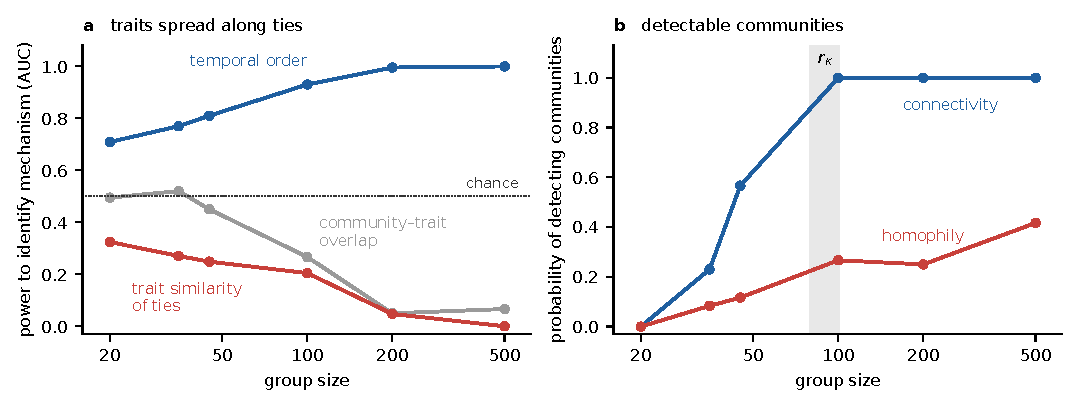
\includegraphics[width=\textwidth]{figs_ms/fig1.pdf}
\caption{Only temporal order identifies the mechanism, and only larger groups show network-grown
communities. Synthetic societies grown by local network rules (connectivity, $\lambda=0$) or by homophily
on a binary trait ($\lambda=1$). (\textit{a}) Power to tell the two apart (AUC; 0.5 is chance, below 0.5
points the wrong way) when traits also spread along ties. Snapshot statistics (similarity of tied
individuals, overlap of communities with traits) point the wrong way; the temporal statistic, similarity
gained after a tie forms, identifies the mechanism. (\textit{b}) Probability that communities are
detected (stochastic block model) against group size. Communities built by local growth appear above
$r_\kappa\approx80$--100 individuals; homophilous groups at the same strength rarely reach detection.
60--100 replicates per point.}
\label{fig:power}
\end{figure}

\subsection{A natural experiment: a chimpanzee community splits}

Group fission is a natural experiment. If communities follow traits, the fission line should follow
traits; if they follow the network, it should follow the pre-existing ties. The Ngogo chimpanzee
community of Kibale, Uganda, about 200 individuals and one of the largest known, divided permanently into
two groups between 2015 and 2018~\cite{Sandel2026}. Using 25 years of social networks combining grooming,
proximity and party membership, we asked how well each candidate predicts which group an individual
joined.

The network predicted the split years before it happened (figure~\ref{fig:human}a). In 2011--2014 a
spectral cut of the social network assigned 86\% of individuals correctly against 56\% by chance, rising
to 90\% for 2012--2014, and a neighbour vote reached a balanced accuracy of 0.93. The signal was present
from 2007--2008, seven years before polarisation. Sex and age predicted nothing (balanced accuracy
0.42--0.54 in every year). The network cut separated the future groups within males (0.94) and within
females (0.92), so the fission line runs across the classic homophily attributes rather than along them.

Where individuals ranged predicted the split even better: the median GPS location of each individual
assigned it perfectly from 2011, when GPS records begin. To ask whether the social network carried
information beyond shared space, we compared pairs of individuals with the same home-range overlap, the
same distance between ranging centres and the same sex combination. At equal space, future groupmates
groomed each other no more than individuals who would end up on opposite sides (difference in log
grooming weight $-0.04$, 95\% confidence interval $-0.14$ to $0.03$; combined layer $-0.30$, $-0.70$ to
$0.01$). The community therefore divided along spatial neighbourhoods that had existed for years, and its
social ties followed those neighbourhoods. It did not divide along sex or age.

\subsection{Human support networks}

We next examined the three public whole-community networks from small-scale human societies with
individual attributes or proximity (figure~\ref{fig:human}b): material support among 108 adults of the
Mayangna/Miskito community of Arang Dak, Nicaragua~\cite{Koster2018}; gift choices in 18 Agta forager
camps, Philippines~\cite{Smith2018Agta}; and friendship and proximity in Hadza forager camps,
Tanzania~\cite{Fedurek2024}. We predicted held-out ties from attributes, from the network's own
structure (degree and closure through shared partners), and from both.

At Arang Dak, attributes (sex, age, wealth, genetic and affinal relatedness, distance) predict support
with AUC 0.75, the network's own structure with 0.83, and both together with 0.85. Kinship is the
largest attribute effect, but kinship is itself a network, grown by descent and marriage. The structure
of the genealogy, the number of kin two people share and their distance in the kin network, predicts
support beyond their pairwise relatedness (AUC gain 0.012, better in 25 of 25 cross-validation folds).
Once the genealogy is in the model, closure in the support network itself adds almost nothing (0.003).
Support thus flows along the kinship network, to the kin of one's kin, and not only to close relatives.
The community's weak block structure aligns with blocks of the kinship network (NMI 0.27 against 0.06 by
chance), not with sex, age or space. Among the Agta, exogenous attributes barely predict gifts (AUC 0.59;
0.50 across camps), whereas the network's structure reaches 0.78. Among the Hadza, proximity and closure
among friends both predict friendship, and together reach 0.79--0.83.

\begin{figure}[t]
\centering
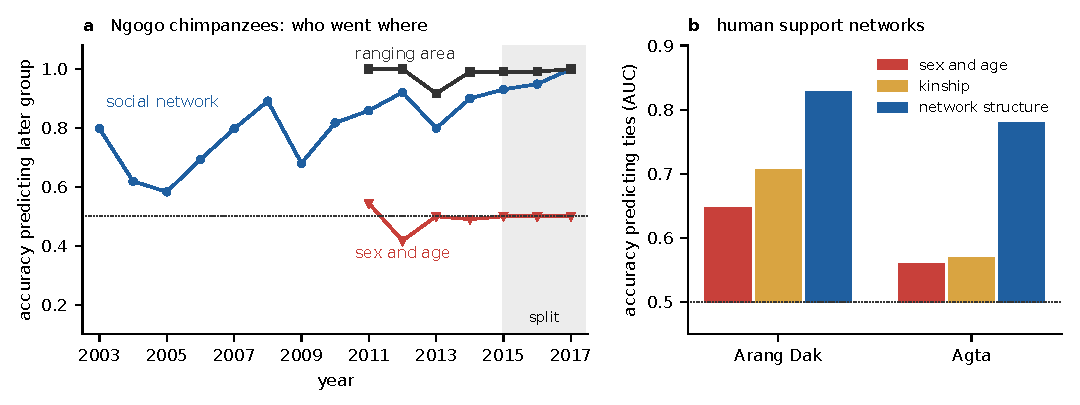
\includegraphics[width=\textwidth]{figs_ms/fig2.pdf}
\caption{Communities do not follow sex or age. (\textit{a}) Ngogo chimpanzees: balanced accuracy with
which each year's data predict the group an individual joined after the 2015--2018 split, from the social
network (neighbour vote), the ranging area (median GPS location, recorded from 2011) and sex and age.
Years with at least 20 labelled individuals. Dotted line, chance. At equal ranging overlap the network
adds nothing (main text). (\textit{b}) Held-out accuracy (AUC) of predicting support or gift ties in two
human communities from sex and age, from kinship, and from the network's own structure (degree and
closure). Dotted line, chance.}
\label{fig:human}
\end{figure}

\subsection{Genetic kinship and culture in prehistoric Europe}

Ancient genomes now reveal who was related to whom across thousands of years. We built networks of
identity-by-descent (IBD) sharing among 705 individuals who lived in Central Europe between the Neolithic
and the Iron Age~\cite{Ringbauer2024,Mallick2024}, and compared them with the archaeological culture of
each burial. Individuals of the same culture are 2.6 times more likely to share IBD than individuals of
different cultures at the same distance and period, well above what spatially contiguous partitions of
the landscape produce (1.3; $P=0.004$). Genetic ties and material culture are thus coupled beyond
geography. The coupling is expected both if similar groups exchanged partners and if groups linked by
marriage came to share material culture. The cross-lagged analysis does not resolve the order at present
sampling densities: the network-first coefficient exceeded the distance-decay and permutation nulls but
not the degree- and edge-length-preserving rewiring ($P=0.63$--0.97 across variants), and depended on a
single cultural transition. The coupling is real, and its direction awaits denser genomic sampling.

\subsection{An arrow of time in the archaeological record}

The decisive test is temporal: do ties come before similarity? The Chaco region of the North American
Southwest offers a rare record. Ceramic assemblages from 280 settlements, dated in 50-year intervals
between AD 800 and 1300~\cite{Mills2018,Daems2023}, allow the similarity of every pair of settlements to
be tracked through the rise and decline of the Chaco system, while the number of settlements grows from
24 to 185 and shrinks again. We defined communities at each time as groups of settlements with similar
assemblages and asked two questions. Does membership of the same community at one time predict that two
settlements will become more similar later? And does the same hold with time reversed?

If community structure were static, with change reflecting only sampling noise, the forward and reversed
effects would be equal. They are not (figure~\ref{fig:chaco}). Settlements in the same community
converged in the following 50 to 100 years, beyond what geography produces, while the time-reversed
effect was zero or negative in every interval. The forward excess was positive in 9 of 10 intervals with
at least 30 settlements, across Chaco and the wider Southwest~\cite{Mills2013}. Under the joint
stationary null, which redraws the whole Chaco series at once so that overlapping intervals remain
dependent as in the data, the mean forward excess over the eight Chaco intervals (0.12) exceeded all 500
null realisations (figure~\ref{fig:chaco}b; $P<0.002$; null 95\% range $-0.04$ to 0.06). It did so both
for consecutive intervals ($P<0.002$) and for intervals 100 years apart, which share no ceramic data
($P=0.01$). Similarity also predicted later community membership beyond earlier membership in 7 of 8
intervals. Connectivity led to similarity, and similarity led to connectivity.

Was the convergence driven by local contact between neighbouring settlements? If so, it should weaken
with distance within a community. It did not: the interaction between shared membership and distance was
indistinguishable from the null ($P=0.19$). Convergence operated at the level of the community as a
whole, over distances of tens of kilometres, as expected for diffusion through a connected network rather
than between adjacent villages.

\begin{figure}[t]
\centering
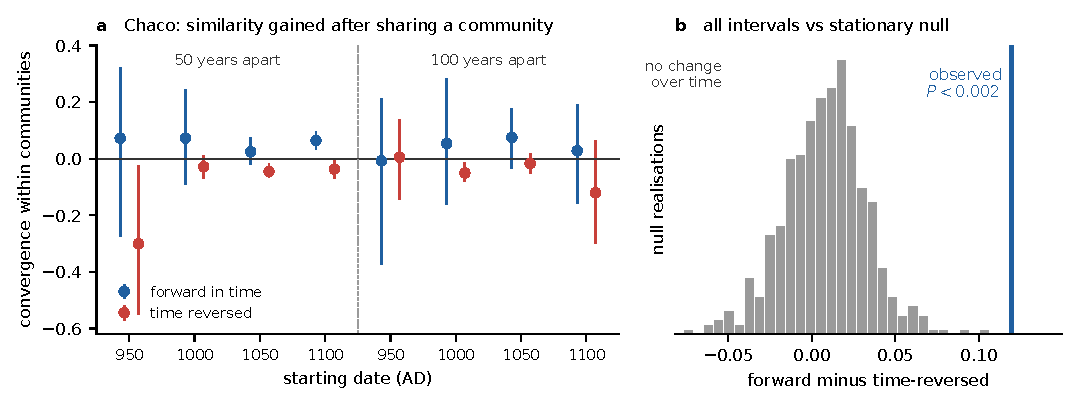
\includegraphics[width=\textwidth]{figs_ms/fig3.pdf}
\caption{Similarity follows connectivity in the Chaco record. (\textit{a}) For each pair of time slices,
the gain in ceramic similarity between settlements that shared a community at the earlier time (blue),
and the same quantity with time reversed (red), controlling for initial similarity, distance and region.
Bars, 95\% node-bootstrap intervals. (\textit{b}) Mean forward-minus-reversed effect over all eight
intervals (blue line) against 500 realisations of a record in which each settlement's composition never
changes (grey).}
\label{fig:chaco}
\end{figure}

%======================================================================
\section{Discussion}

Across a primate community, three human communities, prehistoric genomes and an archaeological time
series, communities are not simply the imprint of shared traits. The traits most often invoked, sex and
age, did not organise the Ngogo fission or human support ties. What did was structure: spatial
neighbourhoods among chimpanzees, the genealogical network among Mayangna households, and, in the Chaco
record, the community structure of the exchange network, which preceded convergence in material culture.
Homophily was present too: similar settlements later joined the same community, and shared culture and
genetic ties went together in prehistoric Europe. Network structure often came first, and the two
mechanisms acted together.

This has a theoretical consequence. If local network growth builds communities on its own, then the
group boundaries of early societies need not have been drawn along pre-existing differences. Instead,
differences such as dialects, styles and customs can accumulate along boundaries that the network
created, and then reinforce them through homophily. Such a feedback would make cultural diversity partly
a consequence of social structure, rather than only its cause. The size threshold of network-grown
communities, about 80 to 100 individuals, sits close to the scale of ancestral bands and villages, and
may have shaped when and where such boundaries first appeared.

The synthetic societies also carry a methodological lesson for studies of small groups. The common
practice of inferring communities and comparing them with attributes has little power below about 80
individuals, and its null results say nothing about mechanism. Dyadic models with the network's own
structure as covariates are informative at much smaller sizes, but under contagion only temporal order
is. Natural experiments such as fissions, and time series such as the archaeological record, are
therefore more valuable than larger snapshots.

The evidence has limits. At Ngogo, spatial and social separation were both present when GPS records
began, so which came first cannot be established. At Arang Dak, the network that matters is the
genealogy, which is also the classic substrate of kin homophily, and the absence of sex and age effects
does not exclude homophily on traits that were not measured. The Chaco communities are defined from
ceramic similarity rather than observed interaction; the arrow of time excludes a static tradition and
spatially local contact, but a regional tradition whose clusters each evolve as a unit would also produce
forward convergence. Only the Chaco record tests temporal order directly. Each limit points to data that
exist: time-stamped proximity networks of forager camps with genealogies~\cite{Migliano2017,Dyble2015},
pedigrees for the Ngogo community, IBD networks from the growing body of ancient genomes, and independent
measures of interaction, such as obsidian sourcing, in the Southwest. These will decide how much of human
social structure the network built for itself.

%======================================================================
\begin{thebibliography}{99}
\setlength{\itemsep}{0pt}\small

\bibitem{McPherson2001}
McPherson M, Smith-Lovin L, Cook JM. 2001 Birds of a feather: homophily in social networks.
\textit{Annu. Rev. Sociol.} \textbf{27}, 415--444.

\bibitem{McElreath2003}
McElreath R, Boyd R, Richerson PJ. 2003 Shared norms and the evolution of ethnic markers.
\textit{Curr. Anthropol.} \textbf{44}, 122--130.

\bibitem{Jin2001}
Jin EM, Girvan M, Newman MEJ. 2001 Structure of growing social networks. \textit{Phys. Rev. E}
\textbf{64}, 046132.

\bibitem{Vazquez2003}
V\'azquez A. 2003 Growing network with local rules: preferential attachment, clustering hierarchy, and
degree correlations. \textit{Phys. Rev. E} \textbf{67}, 056104.

\bibitem{Toivonen2006}
Toivonen R, Onnela J-P, Saram\"aki J, Hyv\"onen J, Kaski K. 2006 A model for social networks.
\textit{Physica A} \textbf{371}, 851--860.

\bibitem{VazquezBook}
[Reference anonymised for review.]

\bibitem{Shalizi2011}
Shalizi CR, Thomas AC. 2011 Homophily and contagion are generically confounded in observational social
network studies. \textit{Sociol. Methods Res.} \textbf{40}, 211--239.

\bibitem{Karimi2018}
Karimi F, G\'enois M, Wagner C, Singer P, Strohmaier M. 2018 Homophily influences ranking of minorities
in social networks. \textit{Sci. Rep.} \textbf{8}, 11077.

\bibitem{Peixoto2014}
Peixoto TP. 2014 Hierarchical block structures and high-resolution model selection in large networks.
\textit{Phys. Rev. X} \textbf{4}, 011047.

\bibitem{Sandel2026}
Sandel AA \textit{et al.} 2026 [Title]. \textit{Science} \textbf{392}, 216--220.

\bibitem{NgogoData}
Sandel AA \textit{et al.} 2026 Ngogo chimpanzee learned social networks, community labels and GPS
subsample. Zenodo. (doi:10.5281/zenodo.19210783; doi:10.5281/zenodo.18626723;
doi:10.5281/zenodo.18603419)

\bibitem{Koster2018}
Koster J. 2018 Family ties: the multilevel effects of households and kinship on the networks of
individuals. \textit{R. Soc. Open Sci.} \textbf{5}, 172159.

\bibitem{KosterData}
Koster J. 2018 Data from: Family ties: the multilevel effects of households and kinship on the networks
of individuals. Figshare. (doi:10.6084/m9.figshare.6056963)

\bibitem{Smith2018Agta}
Smith D \textit{et al.} 2018 A friend in need is a friend indeed: need-based sharing, rather than
cooperative assortment, predicts experimental resource transfers among Agta hunter-gatherers.
\textit{Evol. Hum. Behav.}

\bibitem{AgtaData}
Smith D \textit{et al.} 2018 Data from: A friend in need is a friend indeed. Figshare.
(doi:10.6084/m9.figshare.6960998)

\bibitem{Fedurek2024}
Fedurek P \textit{et al.} 2024 The relationship between perceived friendship and proximity networks
among Tanzanian Hadza. \textit{Hunter Gatherer Res.}

\bibitem{HadzaData}
Fedurek P \textit{et al.} 2024 Data from: The relationship between perceived friendship and proximity
networks among Tanzanian Hadza. Figshare. (doi:10.6084/m9.figshare.24989361)

\bibitem{Ringbauer2024}
Ringbauer H \textit{et al.} 2024 Accurate detection of identity-by-descent segments in human ancient DNA.
\textit{Nat. Genet.} \textbf{56}, 143--151.

\bibitem{ancIBDData}
Ringbauer H \textit{et al.} 2023 ancIBD identity-by-descent segments for 4,248 ancient Eurasians.
Zenodo. (doi:10.5281/zenodo.8417049)

\bibitem{Mallick2024}
Mallick S \textit{et al.} 2024 The Allen Ancient DNA Resource (AADR): a curated compendium of ancient
human genomes. \textit{Sci. Data} \textbf{11}, 182.

\bibitem{AADRData}
Mallick S \textit{et al.} 2024 Allen Ancient DNA Resource. Harvard Dataverse.
(doi:10.7910/DVN/FFIDCW)

\bibitem{Mills2018}
Mills BJ \textit{et al.} 2018 Evaluating Chaco migration scenarios using dynamic social network
analysis. \textit{Antiquity} \textbf{92}, 922--939.

\bibitem{Daems2023}
Daems D, Coco E, Gillreath-Brown A, Kafetzaki D. 2023 The effects of time-averaging on archaeological
networks. \textit{J. Archaeol. Method Theory} \textbf{31}, 473--506.

\bibitem{ChacoData}
Coco E, Daems D \textit{et al.} 2023 time-averaged-networks: Chaco ceramic data. GitHub.
(\url{https://github.com/cocoemily/time-averaged-networks})

\bibitem{Mills2013}
Mills BJ \textit{et al.} 2013 Transformation of social networks in the late pre-Hispanic US Southwest.
\textit{Proc. Natl Acad. Sci. USA} \textbf{110}, 5785--5790.

\bibitem{SWSNData}
Peeples MA \textit{et al.} 2013 SWSN\_2013: Southwest Social Networks similarity matrices. GitHub.
(\url{https://github.com/mpeeples2008/SWSN_2013})

\bibitem{Migliano2017}
Migliano AB \textit{et al.} 2017 Characterization of hunter-gatherer networks and implications for
cumulative culture. \textit{Nat. Hum. Behav.} \textbf{1}, 0043.

\bibitem{Dyble2015}
Dyble M \textit{et al.} 2015 Sex equality can explain the unique social structure of hunter-gatherer
bands. \textit{Science} \textbf{348}, 796--798.

\end{thebibliography}

\end{document}
